\chapter{Some Examples of Markov Chain}
\section{The Simple Random Walk}
The markov chain whose state space is the set of all integers $ \mathds{Z} $ and has transition probabilites
\[
    p_{i,i+1} = p = 1-p_{i,i-1}, \ \ i\in\mathds{Z}.
\]
where $ 0<p<1 $, is called the simple random walk.

\begin{figure}[h]
    \centering
    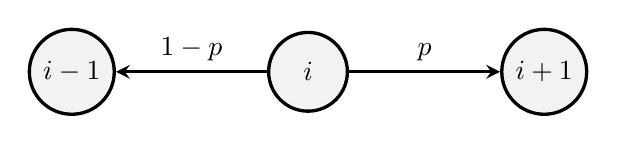
\begin{tikzpicture}[->, >=stealth, auto, very thick, node distance = 3cm, state/.style={circle, draw=black, fill=black!5, very thick, minimum size = 10mm}]
        \node[state] (1) {$i$};
        \node[state] (2) [right of=1] {$i+1$};
        \node[state] (3) [left of=1] {$i-1$};

        \path (1) edge [] node {$p$} (2)
            (1) edge [] node[above] {$1-p$} (3);
    \end{tikzpicture}
    \caption{Simple Random Walk}
    \label{Simple random walk}
\end{figure}

One interpretation is that it represents the winnings of a gambler who on each play of the game either wine or loses one dollar.

Since all state clearly communicate it follows that from \cref{recurent if communicate} they are either all transient or all recurrent. 
So let us consider state 0 and
attempt to determine if  $ \sum_{n=0}^{\infty} p_{00}^{n} $ if finite or not.

Since it is impossible to be back at the initial state after an odd number of transition, we must have,
\[
    p^{2n+1}_{00} = 0 \ \forall n\ge 0.
\]

On other hand, the gambler would be even after $ 2n $ trials if and only if he wens  $ n $ games and lost  $ n $ of games.
It is like coin toss with probability of getting head is $ p $ ans tail in  $ 1-p $. Then the desired probability is those binomial probability.
Then we have,
 \[
     p^{2n}_{00} = \binom{2n}{n}p^{n}(1-p)^{n} = \frac{2n!}{n!n!}(p(1-p))^{n}, \ \ n=1,2,3,\ldots
\]
by using an starling approximation,
i.e.
\[
    n! \sim \sqrt{2\pi n}\left(\frac{n}{e}\right)^{n}.
\]
we obtain 
\[
    p^{2n}_{00}\sim \frac{[4p(1-p)]^{n}}{\sqrt{n\pi}}
\]
we know if $ a_{n}\sim b_{n} $, then $ \sum_{n}a_{n}<\infty  $ iff $ \sum_{n}b_{n}<\infty  $. Consequently $ \sum_{n}p^{n}_{00}<\infty  $ 
if and only if
\[
    \sum_{n=0}^{\infty} \frac{[4p(1-p)]^{n}}{\sqrt{n\pi}} < \infty
\]

However, $ 4p(1-p)\le 1 $ with equality holding if and only if $ p=\frac{1}{2} $. Hence $ \sum_{n=1}^{\infty} p^{n}_{00}=\infty $ 
if and only if $ p=\frac{1}{2} $. Thus, the chain is recurrent with $ p=\frac{1}{2} $ and transient when  $ p\neq \frac{1}{2} $.

Hence, if $ p= 1/2 $ then the process random walk visit state 0 again and again infinitely many time and if  $ p \neq 1/2 $ it may or may 
not visit state 0.

If we consider random walk has  $ N+1 $ step i.e.  $ \{0,1,\ldots,N\} $ is state space of random walk.
Then, The transition matrix will be.
\[
    P = 
    \begin{bmatrix}
        1-p & p & 0 & 0 & \ldots\\ 
        1-p & 0 & p & 0 & \ldots\\ 
        0 & 1-p & 0 & p & \ldots\\ 
        \vdots & \vdots & \vdots & \vdots & \ddots
    \end{bmatrix}_{(N+1)\times(N+1)}
\]
considering $ p_{00} = 1-p $ and $ p_{N N} = p $ as those are last state.

\begin{example}
    Consider a random walk with 4 state and $ p = 0.6 $.\\ 
    Then, the transition probability will be,
    \[
        P = 
        \begin{bmatrix}
            0.4 & 0.6 & 0 & 0\\ 
            0.4 & 0 & 0.6 & 0\\ 
            0 & 0.4 & 0 & 0.6\\ 
            0 & 0 & 0.4 & 0.6
        \end{bmatrix} 
    \]
    then 10000-step transition probability will be
    \[
        P^{10000}=
        \begin{bmatrix}
            0.1231 & 0.1846 & 0.2769 & 0.4154 \\
            0.1231 & 0.1846 & 0.2769 & 0.4154 \\
            0.1231 & 0.1846 & 0.2769 & 0.4154 \\
            0.1231 & 0.1846 & 0.2769 & 0.4154 \\
        \end{bmatrix}
    \]
    hence, Stationary distribution will be 
    \[
        \pi = 
        \begin{bmatrix}
            0.1231 &   0.1846  &  0.2769  &  0.4154
        \end{bmatrix} 
    \]
    As, $ \pi = \pi P $
\end{example}

\subsection{Random Walk in Simulation}
Using python we can simulate a Random Walk. And observing the output we find same result as above. 
If $ p = 0.5 $ the Random walk will visit state 0 over and over again. But it is not the case 
for $ p = 0.6 $ and  $ p = 0.45 $.

\begin{figure}[H]
    \centering
    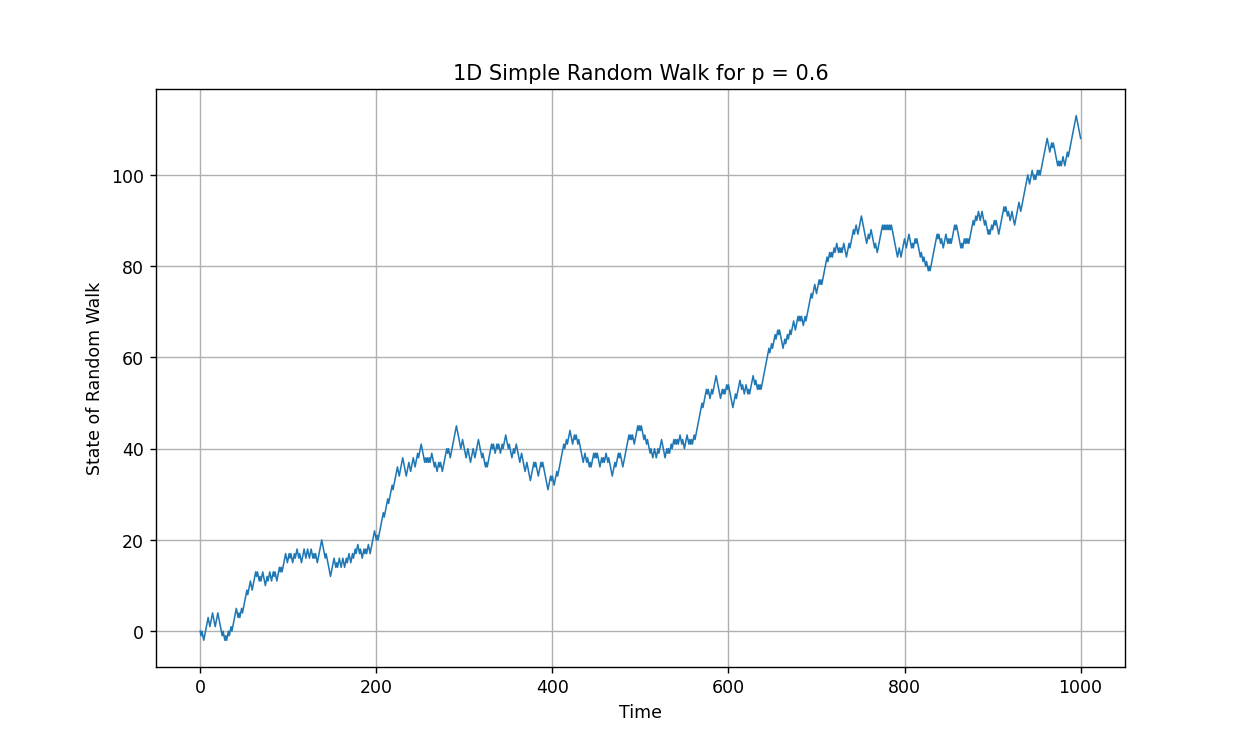
\includegraphics[width=0.7\textwidth]{pic/Random_Walk_0.6.png}
    \caption{Random Walk for $p=0.6$}
    \label{fig:0.6}
\end{figure}
\begin{figure}[H]
    \centering
    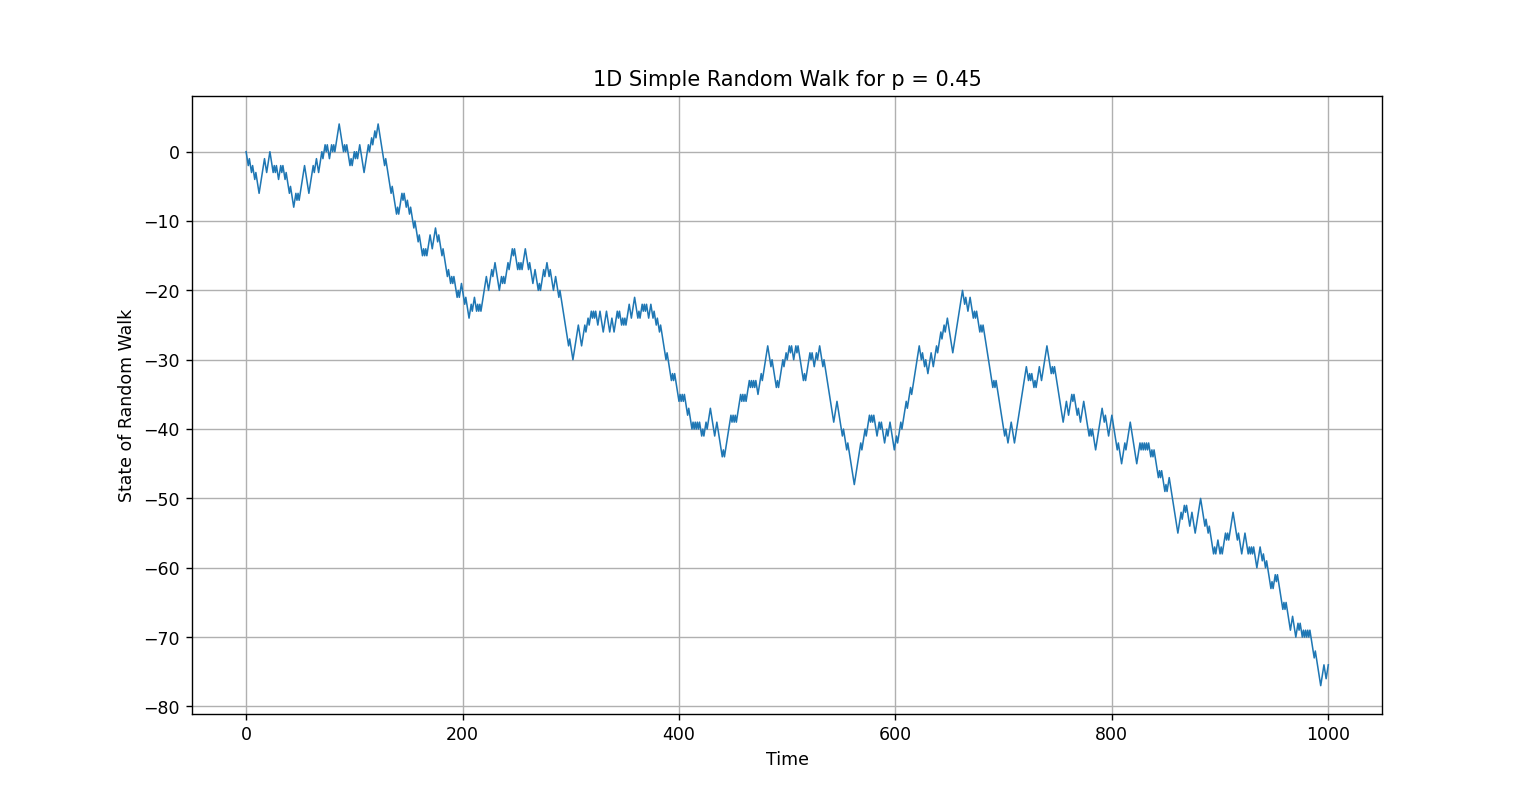
\includegraphics[width=0.7\textwidth]{pic/Random_Walk_0.45.png}
    \caption{Random Walk for $p=0.45$}
    \label{fig:0.45}
\end{figure}


\begin{figure}[H]
    \centering
    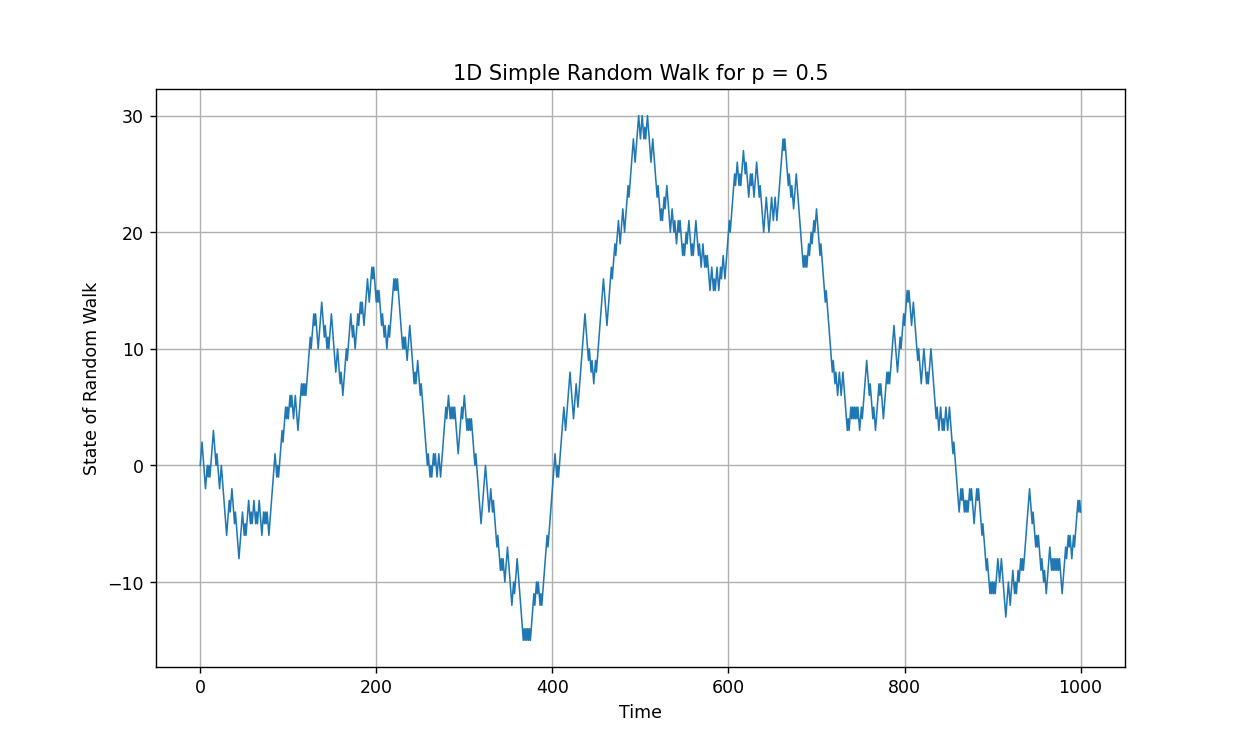
\includegraphics[width=0.7\textwidth]{pic/Random_Walk_0.5.png}
    \caption{Random Walk for $p=0.5$}
    \label{fig:0.5}
\end{figure}

